%!TEX encoding = UTF-8 Unicode
%!TEX root = ../compendium2.tex

\chapter{Integrerad utvecklingsmiljö}\label{appendix:ide}

\section{Vad är en integrerad utvecklingsmiljö?}

En integrerad utvecklingsmiljö \Eng{integrated development environment, IDE} samlar ett flertal verktyg för att skapa, köra och testa program, inklusive en avancerad \textbf{editor} och speciella felsökningsverktyg. % (se appendix \ref{appendix:compile})
 Det finns flera utvecklingsmiljöer att välja mellan, som kan användas för både Scala och Java.

En IDE ger stöd för \textbf{kodkomplettering} \Eng{code completion} där tillgängliga metoder visas i en lista och resten av ett namn kan fyllas i automatiskt efter att du skrivit de första bokstäverna i namnet. En IDE kan hjälpa dig med formatering och även skapa skelettkod utifrån \textbf{kodmallar} \Eng{code templates}. Med \textbf{felindikering} \Eng{error highlighting} får du understrykning av vissa fel direkt i koden och ibland kan du även få hjälp med förslag på åtgärder för att rätta till enkla fel. Funktioner för \textbf{avlusning} \Eng{debugging} hjälper dig att felsöka medan du kör din kod. Med funktioner för \textbf{omstrukturering} \Eng{refactoring} av kod får du hjälp av editorn i samarbete med kompilatorn att göra omfattande strukturförändringar i många kodfiler samtidigt, t.ex. namnbyten med hänsyn taget till språkets synlighetsregler.

Alla dessa avancerade funktioner kan öka produktiviteten avsevärt, men samtidigt tar de tid att lära sig och en IDE kan kräva mycket datorkraft och viss väntetid jämfört med en vanlig, fristående editor. I början kan all funktionalitet upplevas som överväldigande och det kan vara svårt att hitta i alla menyer och inställningar. Det är därför många som föredrar en fristående, snabbstartad kodeditor före en fullfjädrad, tungrodd IDE, speciellt om det rör ett mindre program. Å andra sidan kan en IDE med kodkomplettering vara till stor hjälp när man ska lära sig ett nytt api och experimentera med en okänd kodmassa. Med tiden har hanliga editorer, så som VS Code, fått allt fler  funktioner som tidigiare bara fanns i en fullfjädrad IDE\footnote{Se t.ex. LSP: \url{https://en.wikipedia.org/wiki/Language_Server_Protocol}}, och den praktiska skillnaden allt mindre mellan en ''vanlig'' editor och en IDE blir allt mindre.

I kursen använder vi flera utvecklingsmiljöer. På första labben använder vi Kojo (se appendix \ref{appendix:kojo}) som är en IDE speciellt anpassad på nybörjare. Sedan använder vi en editor t.ex. VS Code, gärna i kombination med byggverktyget \code{sbt}. Du kan under andra halvan av kursen välja att gå över från VS Code till att använda en (annan) IDE, men det går utmärkt att fortsätta med VS Code som numera har en bra debugger för Scala genom tillägget Metals. Om du vill använda en IDE i stället för VS Code så rekommenderas IntelliJ IDEA med Scala-plugin. 
Om du redan lärt dig Eclipse på djupet och verkligen vill fortsätta med denna IDE, välj då ScalaIDE -- dock har denna IDE inte hängt med i den tekniska utvecklingen och ligger kvar på Scala 2.12. 

\section{Visual Studio Code}\label{appendix:ide:vscode}

Visual Studio Code, förkortat VS Code eller bara \code{code}, kallas ofta för ''bara'' en editor, men har genom åren utvecklats till en fullfjädrad IDE med bl.a. inbyggd debugger och stöd för många olika språk via ett omfattande bibliotek av tillägg.%
\footnote{\href{https://en.wikipedia.org/wiki/Visual\_Studio\_Code}{en.wikipedia.org/wiki/Visual\_Studio\_Code}}

Du kan aktivera debuggern i VS Code för dina Scala-program genom att klicka på ''debug'' ovanför din \code{main}-metod, förutsatt att du har tillägget Metals installerad i VS Code och en aktiverad och giltig \code{build.sbt}-fil. Läs mer om debugging i Appendix \ref{appendix:debug}.  


%!TEX encoding = UTF-8 Unicode
%!TEX root = ../compendium2.tex

\section{JetBrains IntelliJ IDEA med Scala-plugin}\label{appendix:ide:intellij}

IntelliJ IDEA%
\footnote{\href{https://en.wikipedia.org/wiki/IntelliJ_IDEA}{en.wikipedia.org/wiki/IntelliJ\_IDEA}}
 är en professionell IDE som stödjer många olika programmeringsspråk. IntelliJ är skriven i Java och utvecklas av det tjeckiska företaget JetBrains.

IntelliJ IDEA finns i två varianter: en gratis gemenskapsvariant med öppenkällkodslicens \Eng{Community edition}, samt en betalvariant med sluten källkod och support-tjänster.


IntelliJ IDEA är en omfattande och avancerad programmeringsmiljö med många funktioner och inställningar. Det finns även en omfattande uppsättning insticksmoduler och tilläggsprogram som underlättar utveckling av t.ex. mobilappar, webbprogram, databaser och mycket annat.

Till IntelliJ IDEA finns en insticksmodul \Eng{plug-in} som stöd för Scala med tillhörande standardbibliotek och byggverktyget \code{sbt}, med mera. Scala-insticksmodulen kan inkluderas genom att välja Scala i en av de dialoger som visas vid första körningen, enligt instruktioner nedan.

I detta avsnitt ges länkar till installation samt tips om hur du kommer igång med att använda IntelliJ IDEA med Scala. Det går ganska snabbt att lära sig grunderna, men det kräven en viss ansträngning att lära sig de mer avancerade funktionerna. Det finns omfattande resurser på nätet som hjälper dig vidare.

Google tillkännagav 2013 att företaget övergår från Eclipse till IntelliJ som den officiellt understödda utvecklingsmiljön för Android och 2014 lanserades utvecklingsmiljön Android Studio%
\footnote {\href{https://en.wikipedia.org/wiki/Android_Studio}{en.wikipedia.org/wiki/Android\_Studio}}
 som bygger vidare på IntelliJ.

\subsection{Installera IntelliJ IDEA}\label{appendix:ide:intellij:install}

IntelliJ med Scala-plug-in är förinstallerat på LTH:s datorer och startas med kommandot \texttt{idea} i ett terminalfönster.

\subsubsection{Ladda ner IntelliJ Scala Bundle (Rekommenderas)}

Om du vill installera IntelliJ med Scala på din egen dator gör du det enklast med paketet \emph{IntelliJ Scala Bundle} via nedan länk för Windows, Mac respektive Linux. Välj senaste versionen med Scala \ScalaVersion.x: 

\url{https://github.com/JetBrains/intellij-scala-bundle/releases} 

Packa upp den nedladdade filen på valfri plats och dubbelklicka på den fil som har ett namn som börjar med \code{idea}. Då kör en färdigkonfigurerad version av IntelliJ igång med ett \code{HelloWorld}-projekt kan startas med Run.

\subsubsection{Installera IntelliJ från grunden}

Om du vill installera IntelliJ från grunden och sedan vid första körningen själv lägga till Scala-plugin gör så här:
\begin{itemize}
  \item För Windows och Mac: ladda ner och kör installationsfil för ditt operativsystem för den öppna varianten kallad \textbf{Community} här: \\
  \url{https://www.jetbrains.com/idea/download/} \\
  Följ instruktionerna som ges av installationsprogrammet.
  
  \item För Ubuntu Linux är det enklast att använda snap-paketet med följande kommando:
\begin{REPLnonum}
sudo snap install intellij-idea-community --classic
\end{REPLnonum}
\item För Ubuntu Linux finns som alternativ till snap-paketet även ett färdigt apt-paket som du kan installera med dessa kommandon i terminalen:
\begin{REPLnonum}
sudo add-apt-repository ppa:mmk2410/intellij-idea-community
sudo apt-get update
sudo apt-get install intellij-idea-community
sudo apt-get upgrade
sudo ln -s /opt/intellij-idea-community/bin/idea.sh /usr/local/bin/idea
\end{REPLnonum}
Det sista kommandot är inte nödvändigt men ger samma startkommando som på skolans datorer. Du kan även starta \textit{IntelliJIDEA Community Edition} via startmenyn genom att söka på intellij.
Mer information om denna ppa finns här:\\ \url{https://launchpad.net/~mmk2410/+archive/ubuntu/intellij-idea-community}

\end{itemize}

\subsection{Anpassa IntelliJ IDEA och installera Scala-plugin}\label{appendix:ide:intellij:tweak}
Om du installerat IntelliJ från grunden får du första gången du kör igång IntelliJ ett antal frågor om vilka anpassningar du vill göra. Följ instruktionerna steg för steg enligt nedan.
\begin{enumerate}

\item Först visas en dialog med titeln \textbf{Complete Installation} som frågar dig om du eventuellt vill importera gamla inställningar eller köra igång med en installation från grunden:
\begin{figure}%[H]
\centering
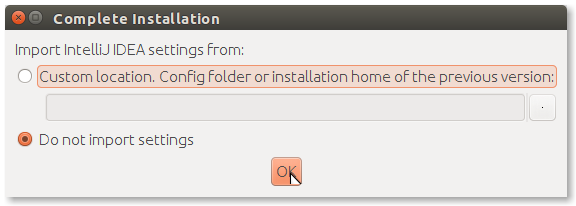
\includegraphics[width=0.75\textwidth]{../img/intellij/idea1-complete-installation.png}
\caption {Första gången får du denna dialog. Klicka \Button{Ok}.}
\label{fig:eclipse:import-projects}
\end{figure}
Om du inte får denna dialog har du troligen en dold katalog i din hemkatalog från en tidigare installation som börjar med namnet \texttt{.Idea} följt av versionnummer. Om du tar bort denna katalog före du kör igång IntelliJ kan du göra om inställningarna från grunden.

\item Efter licensacceptansdialogen kommer fönstret \textbf{Customize IntelliJ IDEA} där du först får välja att ställa in \textbf{UI Theme}. Denna inställning gäller utseende på gränssnittet. Det tema som kallas \textit{Darcula} är en populär variant med mörk bakgrund och nedtonade färger anpassade för att vara skonsamma mot ögonen. Du kan lätt ändra detta val senare. Klicka \Button{Next} när du valt tema.

\item Därefter kan du i fönstret \textbf{Customize IntelliJ IDEA} välja att installera skrivbordsikon och startmenyikon och sedan att skapa ett körskript. Om du kör Linux och installerat IntelliJ enligt föregående avsnitt eller kör på LTH:S datorer har du redan detta och du kan med fördel \textbf{avmarkera dessa val om ikon och startskript} och slippa dubbla ikoner i startmenyn. Kör du Windows eller MacOS kan du i stället med fördel välja installation av startikoner och startskript.

\item \textbf{Default plugins:} \emph{Tune IDEA to your tasks}. Denna dialog gäller inställningar av befintliga insticksmoduler. Dessa inställningar fungerar bra som de är. Klicka \Button{Next}.

\item \textbf{Featured plugins}. I rutan för \textbf{Plugin for Scala language support} Klicka \Button{Install} och låt installationen av Scala fullbordas.

\item När Scala-plugin-installationen är klar, klicka \Button{Start using IntelliJ IDEA}.

\item I välkomstfönstrets nedre hörn, välj \MenuArrow{Configure}\Menu{Settings} och överväg om du vill göra följande lämpliga men ej nödvändiga inställningar.
\begin{enumerate}
\item I fliken \MenuArrow{Editor}\Menu{General} markera \FramedCheckmark{Change font size (Zoom) with Ctrl+Mouse Wheel} för att lätt kunna ändra textstorlek i editorn. Glöm inte att klicka \Button{Apply} nere till höger.

\item I fliken \MenuArrow{Editor}\Menu{Inspections} och välj att expandera \Menu{Spelling} i högra listan. Avmarkera \FramedUnchecked{Typo} för att undvika att svenska ord blir markerade som felstavade. Glöm inte att klicka \Button{Apply} nere till höger.

\item I fliken \MenuArrow{Editor}\Menu{File and Code Templates} och under fliken \Menu{Files} i högra listan: för varje Scala-filtyp (Scala Class, Scala Trait, Scala Object, ...) ta bort andra raden i mallen med texten \code{#parse("File Header.java")} för att slippa onödiga kommentarer i koden när du skapar nya filer. Glöm inte att klicka \Button{Apply} nere till höger. Klicka OK när du är klar med att ändra i \Menu{Settings}.

\end{enumerate}
\end{enumerate}
Du kan också göra ovan och liknande anpassningar senare genom applikationsmenyn \MenuArrow{File}\Menu{Settings...}. Det finns en enorm mängd inställnigar som du kan läsa om i hjälpen som finns på Jetbrains hemsida. Om du vill tillbaka till grundinställningarna kan du ta bort den dolda katalog i din hemkatalog som börjar med namnet \texttt{.Idea} följt av versionnummer och börja om i grundläge vid nästa applikationsstart.





\subsection{Använda IntelliJ IDEA med Scala-plugin}%\label{appendix:ide:intellij:use}

\subsubsection{Skapa ett nytt Scala-projekt}

När du startar IntelliJ IDEA utan förvalt projekt visas välkomstskärmen i figur \ref{fig:idea:welcome}.
\begin{figure}[h]
\centering
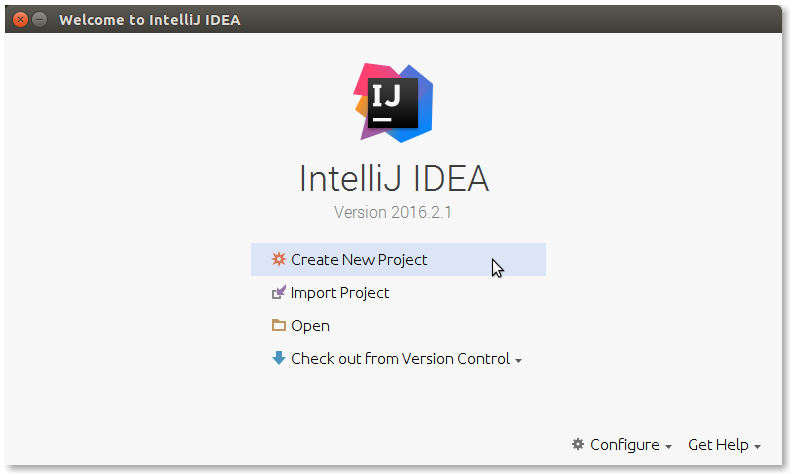
\includegraphics[width=1.0\textwidth]{../img/intellij/idea-welcome.png}
\caption{Välkomstfönstret för IntelliJ IDEA. \label{fig:idea:welcome}}
\end{figure}

\noindent Klicka på \Menu{Create New Project}, varefter dialogen i figur \ref{fig:idea:new-project} visas. Följ stegen enligt nedan.


\begin{enumerate}
\item I dialogen \textbf{New Project} ska du välja projekttyp och körmiljö för ditt projekt enligt figur \ref{fig:idea:new-project}. Välj Scala och SBT och klicka \Button{Next}.

\item Ge projektet namnet \texttt{hello} enligt figur \ref{fig:idea:new-hello-project}.

\begin{figure}[h]
\centering
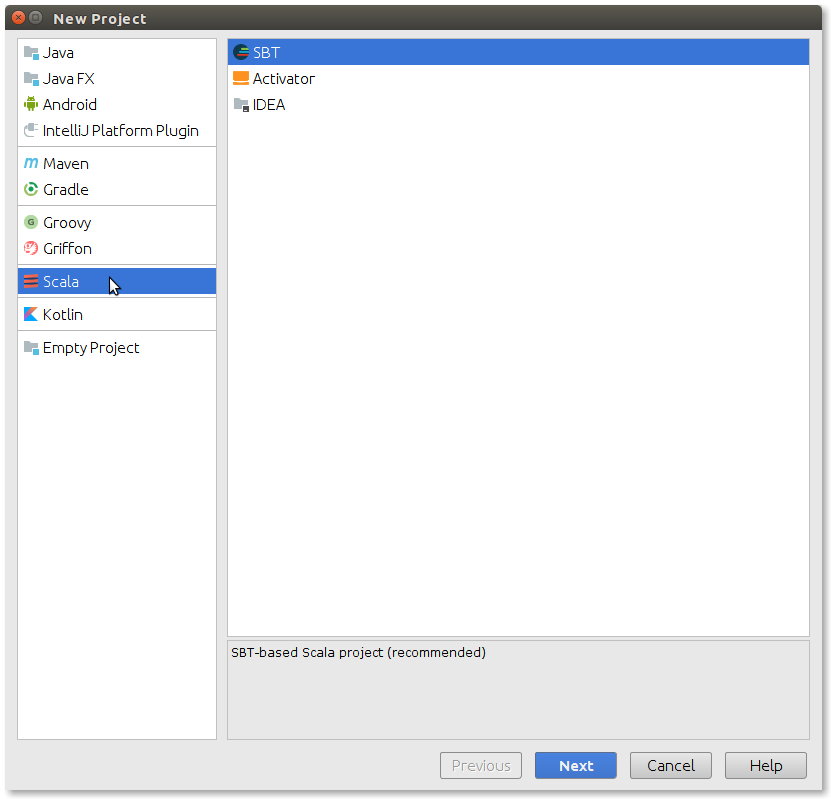
\includegraphics[width=1.0\textwidth]{../img/intellij/idea-new-scala-project.png}
\caption{Välj att skapa ett Scala-projekt med SBT och klicka \Button{Next}.}
\label{fig:idea:new-project}
\end{figure}

\begin{figure}[h]
\centering
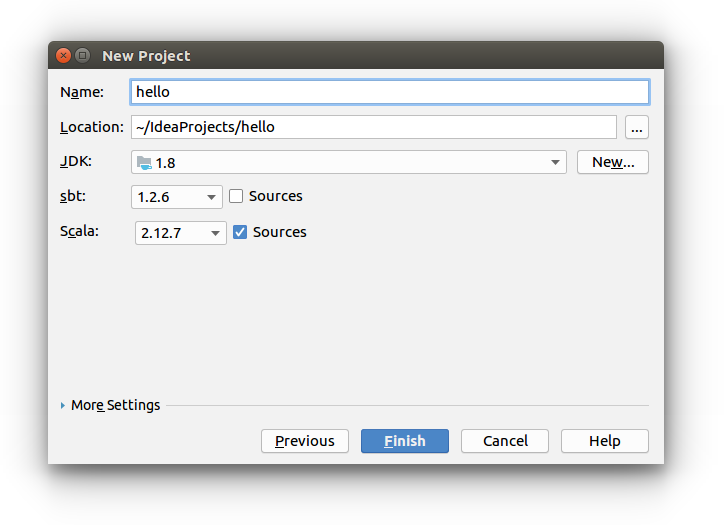
\includegraphics[width=1.0\textwidth]{../img/intellij/idea-new-hello-project.png}
\caption{Ge ditt nya Scala-projekt ett namn, t.ex. \code{hello}. Låt versionsnummer för sbt och Scala vara så som förifyllda (ev. andra versioner än i bilden ovan, beroende på vilken version av IntelliJ du kör.). \label{fig:idea:new-hello-project}}

\end{figure}

\item Avsluta med att klicka \Button{Finish}.

\item Nu öppnas ett projektfönster och det visas även ett välkomstfönster \textit{Tip of the Day} med tips om hur du använder IntelliJ (om du inte stängt av denna funktion). Om du vill kan du läsa igenom några tips nu, eller så kan du stänga fönstret och läsa tipsen nästa gång du öppnar/skapar ett projekt. Tipsen är en god hjälp att komma igång med alla kortkommandon som gör ditt arbete effektivt. %Projektfönstret visas i figur \ref{fig:idea:project-hello}..

% \begin{figure}[H]
% \centering
% 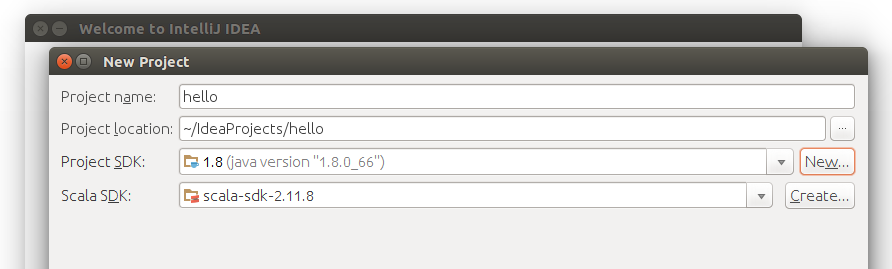
\includegraphics[width=1.0\textwidth]{../img/intellij/idea-new-project.png}
%
% \begin{minipage}{0.27\textwidth}
% 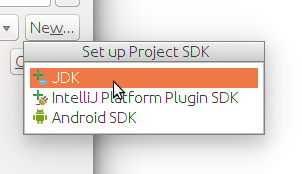
\includegraphics[width=1.0\textwidth]{../img/intellij/idea-project-sdk-jvm.png}
% \end{minipage}
% \begin{minipage}{0.35\textwidth}
% 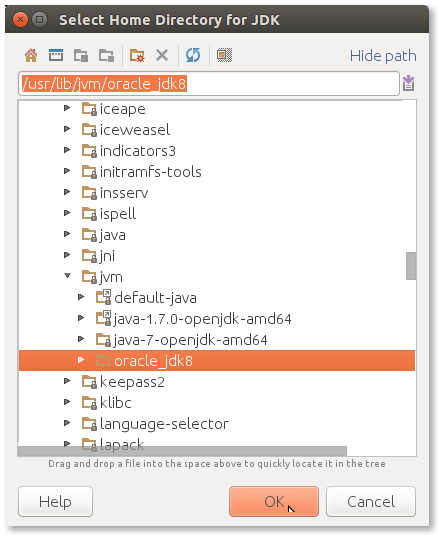
\includegraphics[width=1.0\textwidth]{../img/intellij/idea-project-sdk-home.png}
% \end{minipage}
% \begin{minipage}{0.35\textwidth}
% 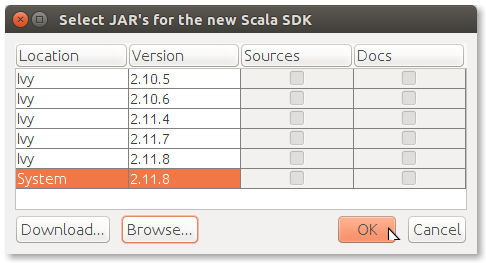
\includegraphics[width=1.0\textwidth]{../img/intellij/idea-scala-sdk.png}
% \end{minipage}%
%
% \caption{Namnge ditt projekt och ställ in körmiljön för JVM och Scala genom att klicka på \Button{New...} och \Button{Create...}}.
% \label{fig:idea:new-project}
% \end{figure}



\begin{figure}
\centering
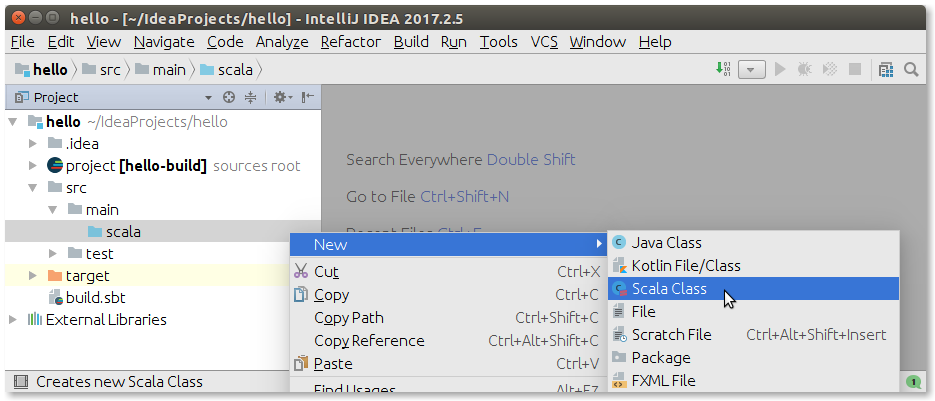
\includegraphics[width=1.0\textwidth]{../img/intellij/idea-new-scala-class.png}

\begin{minipage}{0.35\textwidth}
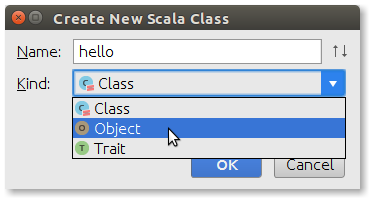
\includegraphics[width=1.0\textwidth]{../img/intellij/idea-scala-object.png}
\end{minipage}
\begin{minipage}{0.60\textwidth}
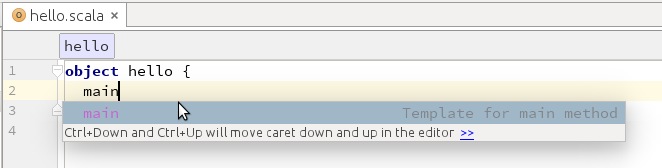
\includegraphics[width=1.0\textwidth]{../img/intellij/idea-complete-main.png}
\end{minipage}%

\caption{Välj \MenuArrow{New}\Menu{Scala Class} genom att högerklicka på  mappen \texttt{src/main/scala} och skapa ett nytt Scala-objekt med \code{main}-metod. Aktivera kodkomplettering i editorn efter ordet \code{main} genom att trycka på TAB-tangenten.}
\label{fig:idea:project-hello}
\end{figure}


\item Första gången ett projekt byggs jobbar IntelliJ IDEA i bakgrunden med att skapa filstruktur och ev. ladda ner de paket som behövs. Denna process kan ta ett tag och när allt är klart står det \textbf{hello: sync finished} nere i \textbf{Build: Sync}-fliken.

\item Klicka på projektmappen \code{hello} och veckla ut mappen \texttt{src/main/scala} och högerklicka på \texttt{scala}-mappen och välj \MenuArrow{New}\Menu{Scala Class}. I dialogen \textbf{Create New Scala Class} välj \emph{Kind:} \textbf{Object} (i stället för Class) och kalla singelobjektet för t.ex. \code{hello} i \emph{Name}-fältet och klicka \Button{OK}, enligt figur \ref{fig:idea:project-hello}.

\item Du får nu upp ett editorfönster med koden för objektet \code{hello}. Skriv ordet \code{main} inuti objektet och tryck TAB för att aktivera kodkomplettering. En mall för \code{main}-metoden klistras då in i objektet.

\item Skriv kod så att det ser ut som i editorfönstret i figur \ref{fig:idea:hello-world} på sidan \pageref{fig:idea:hello-world}.

\item \textbf{Bakgrundsaktiviteter}. Nere i projektföntrets statusområde visas aktiviteter, t.ex. nedladdningar och kompileringar, som pågår i bakgrunden. Du kan ofta arbeta med editering parallellt med bakgrundsaktiviteter, men t.ex. vid körning av program behöver du ibland vänta tills bakgrundsaktiviteterna är klara. Det kan därför vara bra att hålla koll på progress av bakgrundsaktiviteter om du undrar varför du ibland inte får omedelbar respons.


\item Kör igång ditt program genom att klicka på play-knappen eller genom att trycka Shift+F10. Om play-knappen är initialt är grå i stället för grön, välj menyn \MenuArrow{Run}\Menu{Run...}.

\end{enumerate}


\noindent Mer information om hur du använder Scala-plugin för IntelliJ finns här:\\
\href{https://confluence.jetbrains.com/display/SCA/Scala+Plugin+for+IntelliJ+IDEA}{confluence.jetbrains.com/display/SCA/Scala+Plugin+for+IntelliJ+IDEA}

\begin{figure}
\centering
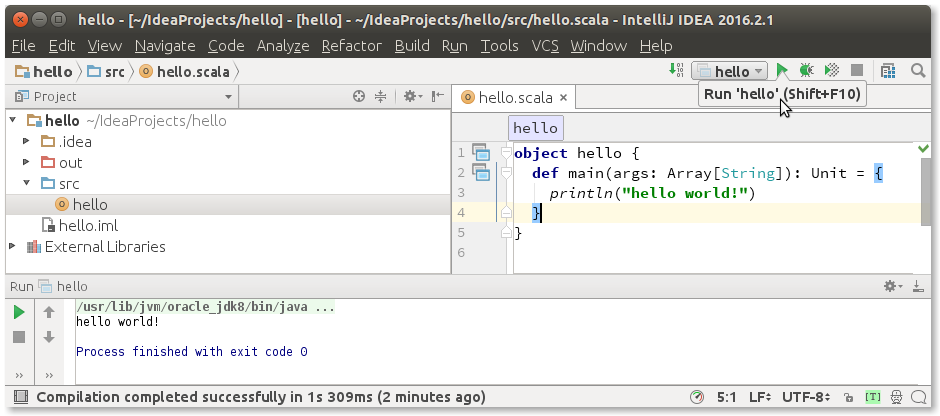
\includegraphics[width=1.0\textwidth]{../img/intellij/idea-hello.png}
\caption{Kör ditt program med play-knappen eller (första gången) välj menyn \MenuArrow{Run}\Menu{Run...} och välj \code{hello}.}
\label{fig:idea:hello-world}
\end{figure}

\clearpage

\subsubsection{Ladda ner kursens workspace och importera i IntelliJ IDEA}

Det finns en zip-fil med ett workspace med projekt för flera av kursens laborationer som du kan ladda ner och importera i Eclipse. Följ stegen nedan.

\begin{enumerate}
\item Ladda ner kursens workspace från \url{http://cs.lth.se/pgk/ws} och Packa upp filen på lämpligt ställe:
\begin{REPLnonum}
> mkdir pgk && cd pgk
> wget -O ws.zip http://cs.lth.se/pgk/ws
> unzip ws.zip
> ls
workspace  ws.zip
\end{REPLnonum}

\item Starta IntelliJ. Om du redan har ett projekt igång välj menyn \MenuArrow{File}\Menu{Close project} så kommer du tillbaka till välkomstfönstret. Välj \textbf{Import Project} så som visas i figure \ref{fig:idea:import1-project}.

\begin{figure}[H]
\centering
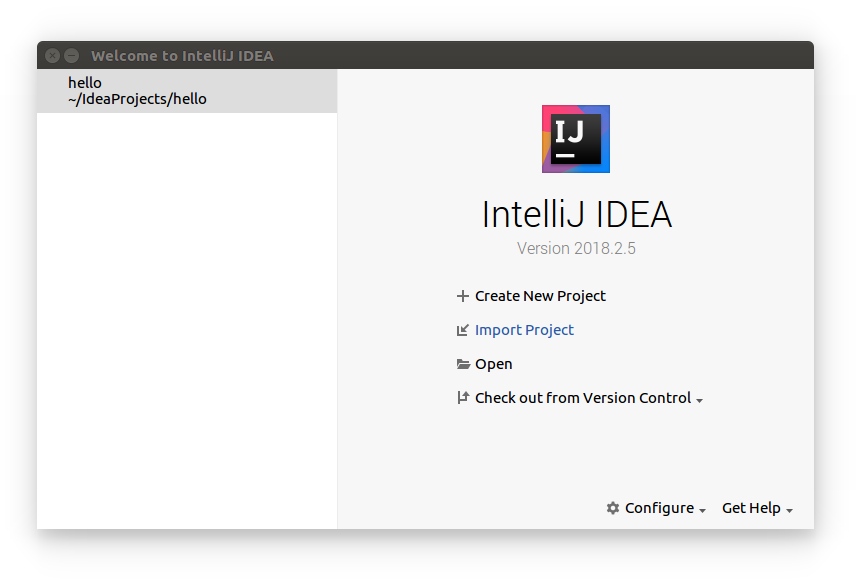
\includegraphics[width=1.0\textwidth]{../img/intellij/idea-import1-project.png}
\caption{Välj \Menu{Import Project} efter att du stängt ev. öppna projekt.}
\label{fig:idea:import1-project}
\end{figure}

\item Bläddra dit du packat upp workspace och markera denna folder i likhet med figur \ref{fig:idea:import23-select} och klicka \Button{OK}. I den efterföljande dialogen välj \textbf{Eclipse} och klicka \Button{Next}.

\item Klicka \Button{Next} igen i dialogen som liknar figur \ref{fig:idea:import4-directory} på sidan \pageref{fig:idea:import4-directory}, där mappen du valt är förvald.

\item Klicka \Button{Next} igen enligt figur \ref{fig:idea:import5-select-projects} på sidan  \pageref{fig:idea:import5-select-projects}. Alla tillgängliga Eclipse-projekt ska vara markerade.

\item Klicka \Button{Next} igen enligt figur \ref{fig:idea:import6-code-style} och sedan  \Button{Finish} enligt figur \ref{fig:idea:import6-select-SDK} med förifylld text oförändrad.

\item Följ instruktionerna i figur \ref{fig:idea:import78-setup-scala-sdk} på sidan \pageref{fig:idea:import78-setup-scala-sdk} för att klicka på \textbf{Setup Scala SDK} och sedan köra \code{Main} i projektet \code{w08_life}.

\end{enumerate}

\noindent Om du får problem på vägen, be någon med erfarenhet av IntelliJ om hjälp.


%{\vfill
\begin{figure}[h]
\centering
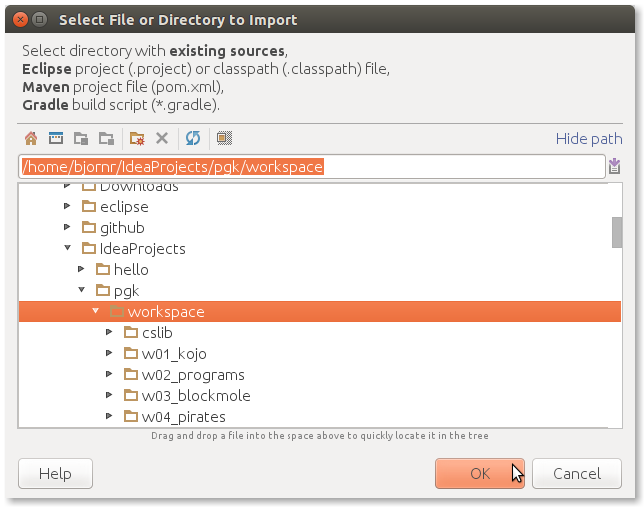
\includegraphics[width=0.5\textwidth]{../img/intellij/idea-import2-select.png}%
\hfill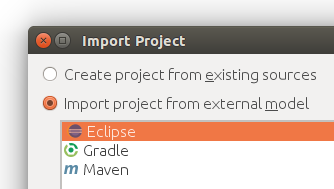
\includegraphics[width=0.4\textwidth]{../img/intellij/idea-import3-eclipse.png}

\caption{Markera den upp-packade workspace-mappen från zip-filen som du laddat ner från: \url{http://cs.lth.se/pgk/ws} och välj \textbf{Eclipse}-import.}
\label{fig:idea:import23-select}
\end{figure}
%}

\begin{figure}[h]
\centering
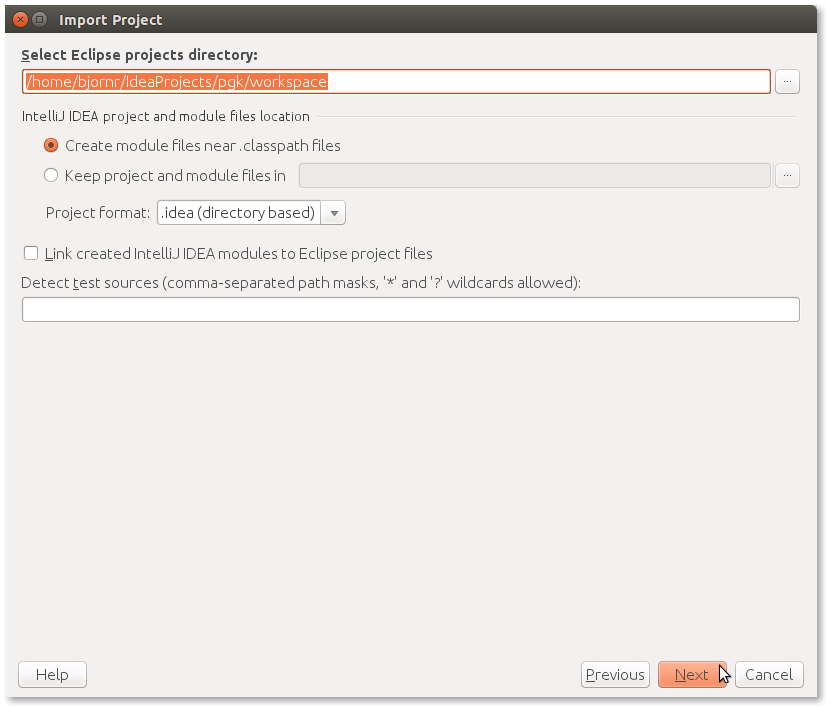
\includegraphics[width=0.7\textwidth]{../img/intellij/idea-import4-directory.png}
\caption{Klicka \Button{Next} med förvalda alternativ oförändrade.}
\label{fig:idea:import4-directory}
\end{figure}

\begin{figure}
\centering
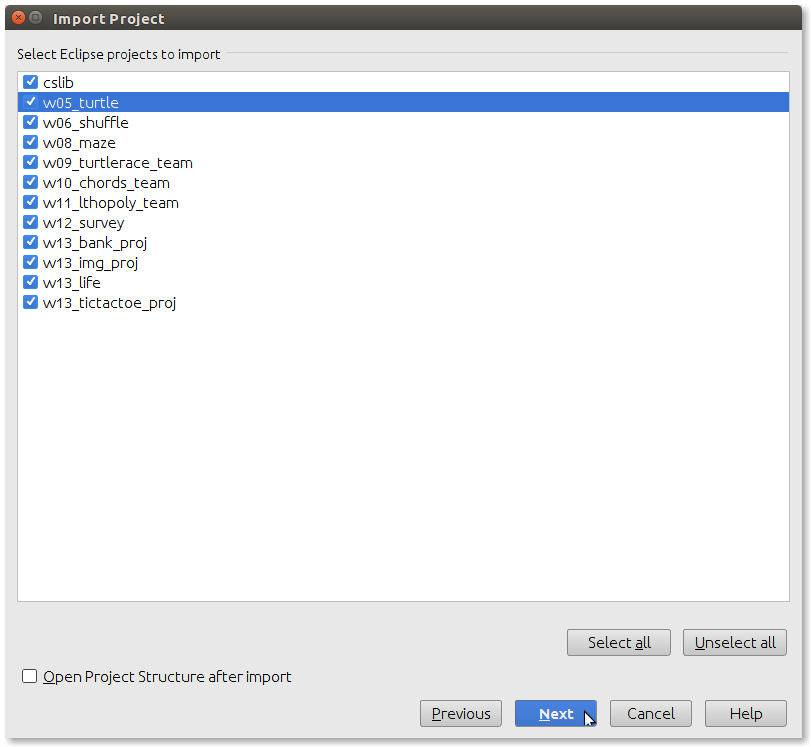
\includegraphics[width=0.8\textwidth]{../img/intellij/idea-import5-select-projects.png}
\caption{Klicka \Button{Next} med alla projekt markerade.}
\label{fig:idea:import5-select-projects}
\end{figure}

\begin{figure}
\centering
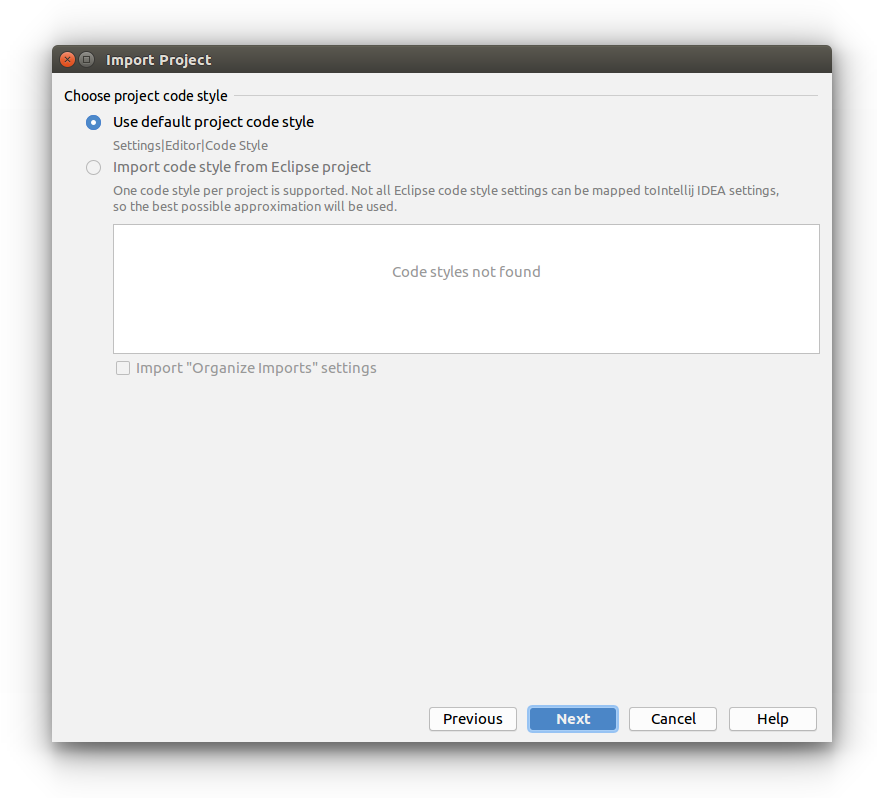
\includegraphics[width=0.8\textwidth]{../img/intellij/idea-import6-code-style.png}
\caption{Klicka \Button{Next} med alla projekt markerade.}
\label{fig:idea:import6-code-style}
\end{figure}


\begin{figure}
\centering
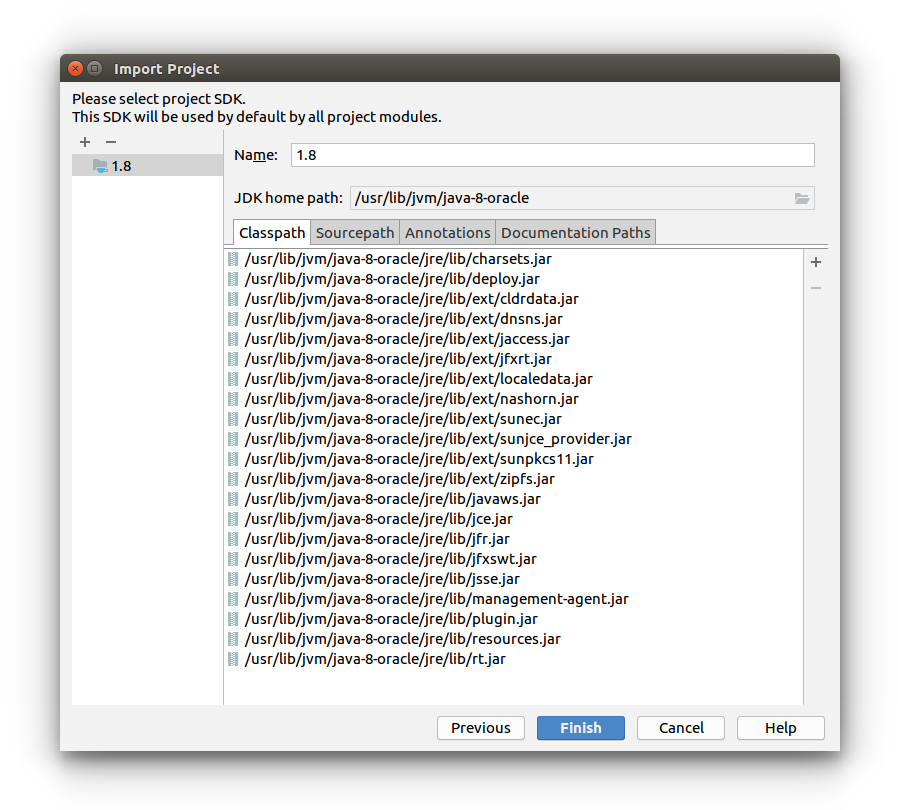
\includegraphics[width=0.8\textwidth]{../img/intellij/idea-import6-select-SDK.png}
\caption{Klicka \Button{Finish} med förifyllda fält oförändrade.}
\label{fig:idea:import6-select-SDK}
\end{figure}

\begin{figure}
\centering
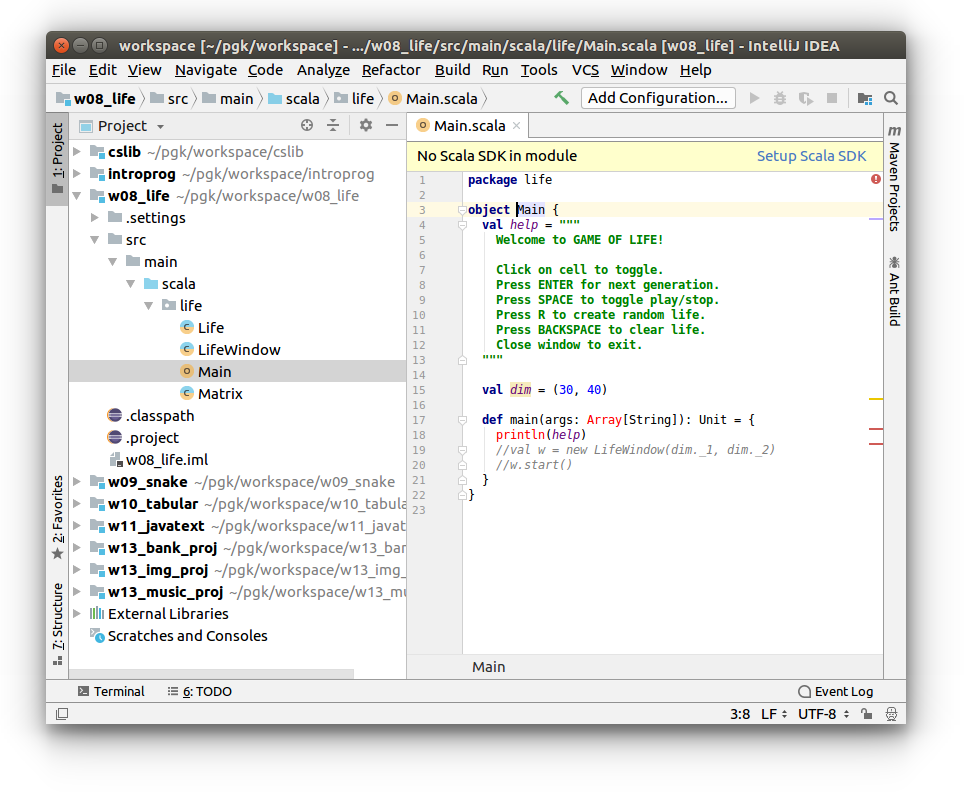
\includegraphics[width=0.8\textwidth]{../img/intellij/import78-setup-scala-sdk.png}

\caption{Bläddra fram till \code{Main}-objektet i projektet \code{w08_life} och klicka på länken \textbf{Setup Scala SDK} i det gula fältet och klicka \Button{Create...} och välj t.ex. \emph{System Version 2.12.8} så att det står t.ex. \code{scala-sdk-2.12.8} som ''Use library'' i efterföljande dialog. Upprepa samma procedur för \emph{Setup SDK} för \code{PixelWindow} i projektet \code{introprog}. Höger-klicka på \code{Main}-objektet i projektet \code{w08_life} och välj \Menu{Run}. När bygget är klart ska en hjälp-utskrift visas.}
\label{fig:idea:import78-setup-scala-sdk}
\end{figure}


% \clearpage
%
% \subsection{Använda debuggern i IntelliJ IDEA med Scala-plugin}
%
% !!! Läs först appendix \ref{appendix:debug}
%
% \subsubsection{Sätta brytpunkter i IntelliJ}\TODO
% \subsubsection{Stegad exekvering i IntelliJ}\TODO
% \subsubsection{Inspektera variabler i IntelliJ}\TODO


% \newpage

% %!TEX encoding = UTF-8 Unicode
%!TEX root = ../compendium2.tex

\section{ScalaIDE och Eclipse}\label{appendix:ide:eclipse}

\begin{oframed}
  \noindent \textbf{OBS!} Eclipse-stödet för Scala har på senare tid inte hängt med i den tekniska utvecklingen och Eclipse med ScalaIDE \ScalaIDEVersion~ligger kvar på gamla Scala 2.12. Om du inte av speciella skäl (t.ex. att du redan lärt dig Eclipse på djupet) vill använda Eclipse, så rekommenderas i stället VS Code eller IntelliJ.  
  \end{oframed}
  

Eclipse%
\footnote{\href{https://en.wikipedia.org/wiki/Eclipse_(software)}{en.wikipedia.org/wiki/Eclipse\_(software)}}
är en professionell IDE som stödjer många olika programmeringsspråk. Eclipse är skriven i Java och bygger vidare på ett utvecklingsprojekt som initierades av IBM. Eclipse är ett fritt och öppet projekt som numera kontrolleras av en oberoende stiftelse.

Till Eclipse finns en insticksmodul \Eng{plug-in} som kallas ScalaIDE och erbjuder stöd för Scala med tillhörande standardbibliotek.

Eclipse är en omfattande och avancerad programmeringsmiljö med många funktioner och inställningar. Det finns även en omfattande uppsättning insticksmoduler och tilläggsprogram som underlättar utveckling av t.ex. webbprogram, databaser och mycket annat.

I detta avsnitt ges länkar till installation samt tips om hur du kommer igång med att använda Eclipse och ScalaIDE. 

%Det går ganska snabbt att lära sig grunderna, men det kräven en viss ansträngning att lära sig de mer avancerade funktionerna. Det finns omfattande resurser på nätet som hjälper dig vidare.


\subsection{Installera ScalaIDE}\label{appendix:ide:eclipse:install}

Eclipse med ScalaIDE är förinstallerat på LTH:s datorer och startas med kommandot \texttt{scalaide} i ett terminalfönster.
För att installera ScalaIDE på din egen dator, följ nedan instruktioner:

\begin{enumerate}
\item Kontrollera enligt avsnitt \ref{appendix:compile:check-jdk} att du har \texttt{java} installerat och installera vid behov JDK enligt avsnitt \ref{appendix:compile:install-jdk}.

\item Installera senaste version av ScalaIDE (i skrivande stund \ScalaVersion för Eclipse Oxygene och Scala 2.12.3) från denna sida:  \url{http://scala-ide.org/download/sdk.html} \\
Följ dessa steg:
\begin{enumerate}
\item Klicka på den variant som passar ditt operativsystem.
\item Filen som laddas ner heter något som liknar (beroende på OS): \\ till exempel  \emph{Windows 64-bit}
\\ Det kan ta ett tag att ladda ner filen som är på ca 280MB.

\item Dubbelklicka på filen för att packa upp den, vilket kan ta många minuter. Du får, när up	packningen är klar, en katalog med namnet \code{eclipse} med en fungerande Eclipse-installation som du kan placera var du vill.
\end{enumerate}

\item Kör igång ScalaIDE första gången för att se så det fungerar genom att dubbelklicka på den exekverbara filen som ligger i underkatalogen \texttt{eclipse}. I Windows heter den \texttt{eclipse.exe} medan den exekverbara filen i Linux heter \texttt{eclipse} utan filändelse.

% \item För Ubuntu Linux finns kompletterande installationsanvisningar här, som beskriver hur man kan skapa en ikon i app-menyn m.m.:
% \\ \url{http://askubuntu.com/questions/26632/how-to-install-eclipse}
% \\ Instruktionerna för Linux å länken ovan är nedan anpassade för version 4.6.1 av ScalaIDE som en serie kommandon att köra i terminalen. Adressen är hämtad från \url{http://scala-ide.org/download/sdk.html} genom att högerklicka på nedladdningsknappen och välja kopiering av adressen. Denna adress står efter \code{wget} nedan (anpassa adressen vid behov till nyare version om sådan kommit sedan detta skrevs). Klistra in ett kommando i taget och kontrollera att det inte blir några fellmeddelande. Nedladdningen med \texttt{wget} kan ta ett tag.
% \begin{verbatim}
% $ cd ~/Downloads
% $ wget http://downloads.typesafe.com/scalaide-pack/\
% 4.6.1-vfinal-neon-212-20170609/scala-SDK-4.6.1-vfinal-\
% 2.12-linux.gtk.x86_64.tar.gz
% $ tar -zxvf scala-SDK-4.6.1-vfinal-2.12-linux.gtk.x86_64.tar.gz
% $ sudo mv ~/Downloads/eclipse /opt/scalaide46  # ändra 46 vid behov
% $ cat > ~/Desktop/scalaide.desktop <<EOF
% [Desktop Entry]
% Name=ScalaIDE
% Type=Application
% Exec=env UBUNTU_MENUPROXY=0 scalaide
% Terminal=false
% Icon=scalaide
% Comment=Integrated Development Environment
% NoDisplay=false
% Categories=Development;IDE;
% Name[en]=ScalaIDE
% EOF
% $ chmod +x ~/Desktop/scalaide.desktop
% $ sudo ln -s /opt/scalaide46/eclipse /usr/local/bin/scalaide
% $ sudo desktop-file-install ~/Desktop/scalaide.desktop
% $ sudo cp /opt/scalaide46/icon.xpm /usr/share/pixmaps/scalaide.xpm
% \end{verbatim}
\end{enumerate}


\subsection{Använda ScalaIDE och Eclipse}\label{appendix:ide:eclipse:use}

Ett grundläggande koncept i Eclipse är \textbf{workspace}. Ett workspace utgör ett arbetsområde kopplat till en katalog i ditt filsystem där du kan arbeta med ett eller flera \textbf{projekt}. Ett projekt innehåller i sin tur dina källkodsfiler och klassfiler etc. i en specifik katalogstruktur som Eclipse skapar när du editerar, kompilerar och kör dina projekt.

\subsubsection{Starta och välja workspace}\label{subsubsection:start:eclipse}

När du startar Eclipse måste du välja vilket workspace du vill använda innan du kommer vidare. När du kör igång Eclipse första gången, klicka OK enligt det förslag som ges. Du kan senare växla workspace genom menyn \MenuArrow{File}\Menu{Switch Workspace}. Om katalogen du anger inte redan finns, kommer den att skapas och initieras med de filer Eclipse behöver.

% I figur \ref{fig:appendix:eclipse:welcome} visas välkomstfliken i Eclipse med sina länkar till funktionsöversikt och olika handledningar. Stäng välkomstfliken genom att klicka på flikens kryss eller på ikonen \textit{Workbench}. Då kommer du vidare till den normala arbetsytan i Eclipse. Du kan få tillbaka välkomstfliken igen via menyn \MenuArrow{Help}\Menu{Welcome}.
%
% \begin{figure}[H]
% \centering
% 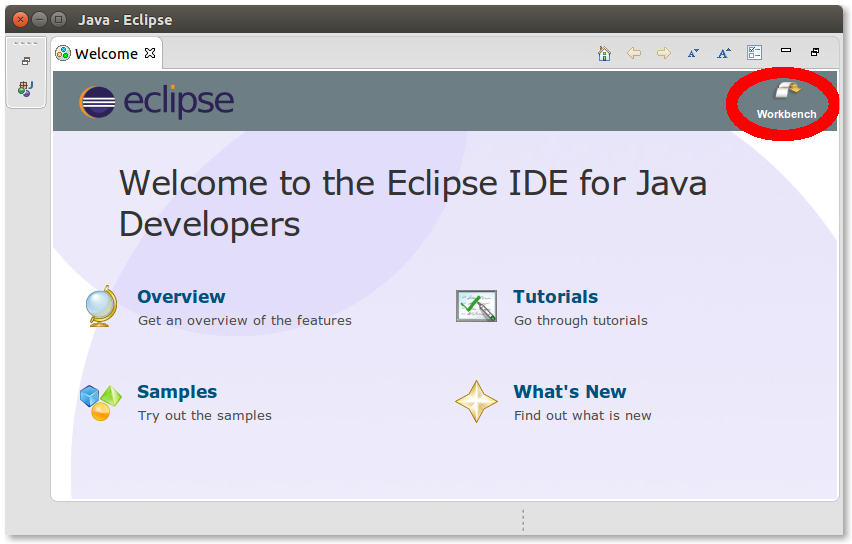
\includegraphics[width=1.0\textwidth]{../img/eclipse/eclipse-welcome.png}
% \caption{Välkomstfliken för Eclipse, som nås via menyn \MenuArrow{Help}\Menu{Welcome}. Gå vidare genom att klicka på \textit{Workbench}.}
% \label{fig:appendix:eclipse:welcome}
% \end{figure}

\subsubsection{Välja perspektiv och visa olika vyer}

Eclipse-fönstret kan innehålla många underfönster i olika flikar, så kallade \textbf{views} eller vyer, som kan arrangeras på olika vis efter hur du vill ha dem. Vilka vyer som syns och hur de placeras beror på vilket s.k. \textbf{perspective} som är aktivt.  Figur \ref{fig:appendix:eclipse:open-perspective} visar arbetsytan med olika vyer i Scala-perspektivet.

Stäng vyn \textit{Outline} om du vill ha mer plats till de övriga vyerna för paketnavigering, editering och utdata. Du kan öppna stängda vyer igen genom menyn \MenuArrow{Window}\Menu{Show View}.
Du kan även återställa perspektivet om din vy blivit konstig med \MenuArrow{Window}\MenuArrow{Perspective}\MenuArrow{Reset Perspective...}

Om du vill anpassa arbetsytan för Java kan du byta perspektiv med klick på 
\includegraphics[scale=0.75]{../img/eclipse/eclipse-perspective-button.png} eller genom menyn \MenuArrow{Window}\MenuArrow{Perspective}\MenuArrow{Open Perspective}\MenuArrow{Other...}\Menu{Java}.

\begin{figure}
\centering
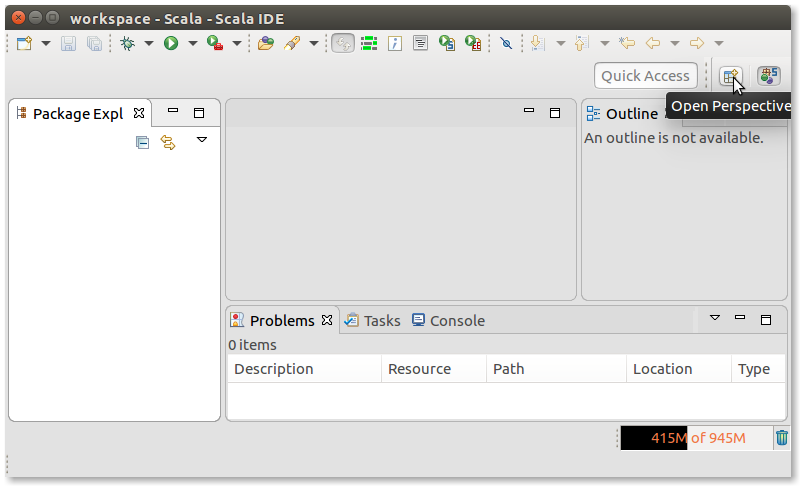
\includegraphics[width=1.0\textwidth]{../img/eclipse/eclipse-scala-perspective.png}
\caption{Arbetsytan i Eclipse. Du kan växla mellan Scala-perspektivet och andra perspektiv, t.ex. Debug-perspektivet eller Java-perspektivet genom att klicka på knappen \Menu{Open Perspective}.}
\label{fig:appendix:eclipse:open-perspective}
\end{figure}

\subsubsection{Hello World}\label{subsubsection:eclipse:hello-world}

Efter att du öppnat ScalaIDE i ett tomt workspace med Scala-perspektivet enligt föregående avsnitt, kan du skapa ditt första projekt med ett \textit{''Hello World''}-program enligt stegen nedan.

\begin{enumerate}
\item Högerklicka i \Menu{Package Explorer} och välj \MenuArrow{New}\Menu{Scala Project}, varefter en dialogruta visas.

\item Fyll i namnet \texttt{hello} i fältet \Menu{Project Name} och klicka \Button{Finish}. Vänta tills skapandet av projektet är klart enligt notifieringar i fönstrets nederkant.

\item Högerklicka igen i \Menu{Package Explorer} och välj \MenuArrow{New}\Menu{Scala Object}, varefter en ny dialogruta visas.

\item Fyll i namnet \texttt{hi} i fältet \Menu{Name} och klicka \Button{Finish}.

\item Du får nu i editorvyn ett kodskelett med \code{object hi}.

\item Börja skriv \code{main} som visas i figur \ref{fig:appendix:eclipse:complete-main} och tryck Ctrl+Mellanslag för att aktivera kodkomplettering \Eng{code completion}. Då får du upp en lista med många alternativ. Välj alternativet \texttt{main - main} varefter ett kodskelett med en main-metod klistras in automatiskt i din kod.

\begin{figure}
\centering
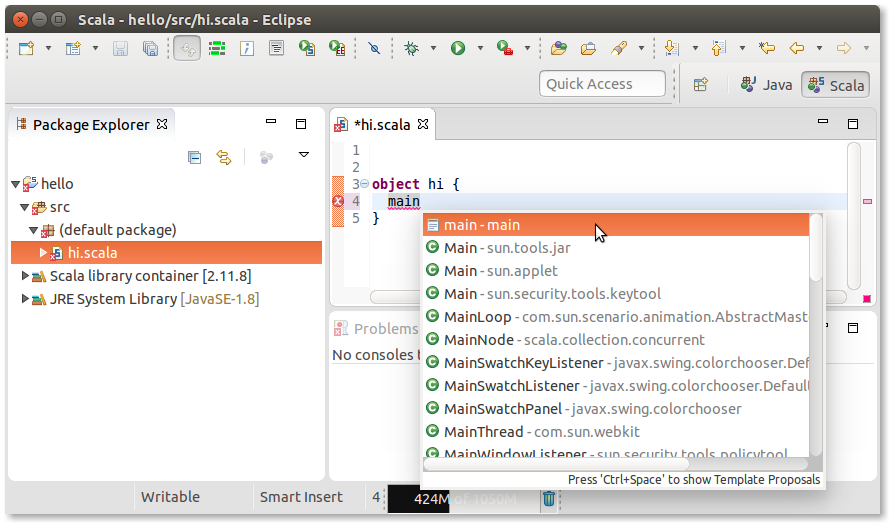
\includegraphics[width=1.0\textwidth]{../img/eclipse/eclipse-complete-main.png}
\caption{Aktivera kodkomplettering med Ctrl+Mellanslag efter ordet \code{main}.}
\label{fig:appendix:eclipse:complete-main}
\end{figure}

\item Fyll i lämplig utskriftstext i ett \code{println}-anrop så att din \code{main}-metod blir så som visas i editorfliken i figur \ref{fig:appendix:eclipse:hello-world}.

\begin{figure}[H]
\centering
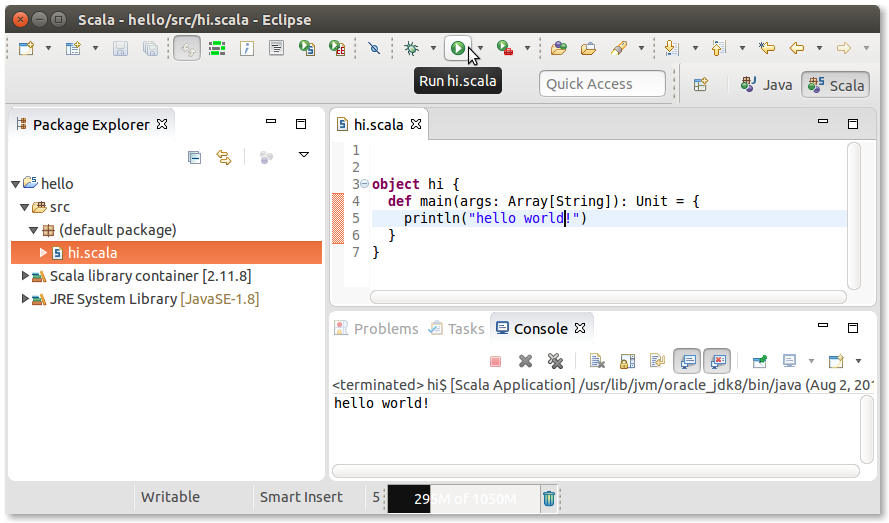
\includegraphics[width=1.0\textwidth]{../img/eclipse/eclipse-hello-world.png}
\caption{Skriv klart \code{main}-metoden och kör ditt program med play-knappen.}
\label{fig:appendix:eclipse:hello-world}
\end{figure}

\item Kör ditt program genom att klicka på den lilla ner-pilen som finns \emph{bredvid} den gröna play-knappen, som muspekaren i figur \ref{fig:appendix:eclipse:hello-world} pekar på. Då vecklas en meny ut där du kan välja \MenuArrow{Run As...}\Menu{Scala Application}. Eller så kan du höger-klicka på filen \texttt{hi.scala} och välja \MenuArrow{Run As...}\Menu{Scala Application}. Detta behöver du bara göra första gången och då skapas en s.k. \textit{Run Configuration}. Du kan sedan trycka Ctrl+F11 för att köra igång din app enligt senaste \textit{Run Configuration} eller klicka på den gröna play-knappen.

\item Du kan öppna din \textit{Run Configuration} genom menyn  \MenuArrow{Run}\Menu{Run Configurations...} och där ställa in många saker, bland annat vilka argument som ska ges till \code{main}-metoden under fliken \textit{Arguments} i textrutan \textit{Program Arguments}.

\end{enumerate}



\subsection{Anpassa ScalaIDE och Eclipse}\label{subsection:appendix:ide:eclipse:tweaks}

\newcommand\EclipsePrefs{\MenuArrow{Window}\MenuArrow{Preferences}}
\newcommand\EclipsePrefsGeneral{\EclipsePrefs\MenuArrow{General}}


%Förutom maxminneshöjningen i filen \texttt{eclipse.ini}, som finns i installationskatalogen för Eclipse, till minst \texttt{-Xmx1G}
Det kan vara bra att göra några ytterligare anpassningar av Eclipse och ScalaIDE enligt nedan. Du hittar inställningarna i menyn \EclipsePrefs ... uppe till höger i Eclipse-fönstret.

\begin{enumerate}
% \item \EclipsePrefsGeneral
% \\ Markera \FramedCheckmark{Show Heap Status} så får du se minnesanvändningen i en liten ruta i nederdelen av fönstret, vilket hjälper dig att upptäcka om minnesbegränsningen i filen \texttt{eclipse.ini} är en flaskhals vid stora projekt och många öppna fönster. Klicka sedan \Button{Apply} längst ner.

% \item \label{item:scala-perspective} \EclipsePrefsGeneral\MenuArrow{Editors}\MenuArrow{Perspectives}
% \\ Markera \textit{Scala} i listan med perspektiv och klicka på knappen
%  \\ \Button{Make default} till höger och sedan på knappen \Button{Apply} längst ner.

\item \EclipsePrefsGeneral\MenuArrow{Editors}\MenuArrow{TextEditors}
\\ Markera \FramedCheckmark{Insert spaces for tabs} så att du slipper specialtecken som kan tolkas olika av olika editorer. Klicka sedan \Button{Apply} längst ner.

\item \EclipsePrefsGeneral\MenuArrow{Editors}\MenuArrow{TextEditors}
\\ \MenuArrow{Spelling} Avmarkera \FramedUnchecked{Enable spell checking} för att slippa att svenska namn och svenska kommentarer markeras som felstavade. Om du senare jobbar med ett projekt helt på engelska, kan du med fördel markera denna kryssruta igen. Klicka sedan \Button{Apply} längst ner.

\item \EclipsePrefsGeneral\MenuArrow{Editors}\MenuArrow{Webbrowser}
\\ Markera \FramedCheckmark{Use external web browser} för att köra din vanliga webbläsare när du klickar på länkar. Klicka sedan \Button{Apply} längst ner.

\item  \EclipsePrefs\MenuArrow{Scala}\MenuArrow{Compiler}
\\ I fliken \textbf{Standard} markera dessa kryssrutor för att få extra varningar: \\
\begin{tabular}{l @{}l @{}l}
\textit{deprecation} & \FramedCheckmark{} & varnar vid användning av föråldrad kod som snart utgår \\
\textit{feature}     & \FramedCheckmark{} & påminner om import vid användning av avancerad kod  \\
\textit{unchecked}   & \FramedCheckmark{} & ger tips vid speciella problem med generiska typer \\
\end{tabular}\\
och klicka sedan på knappen \Button{Apply} längst ner.

\item \EclipsePrefs\MenuArrow{Java}\MenuArrow{Compiler}\MenuArrow{Errors/Warnings}
\\ Veckla ut listan \textbf{Potential programming problems} och sätt \textbf{Resource leak} till alternativet \textbf{Ignore}, så slipper du varningar vid användning \jcode{Scanner} i Java. Klicka sedan \Button{Apply} längst ner.

\end{enumerate}

\noindent Ovan anpassningar är rekommenderade men inte nödvändiga och du kan gärna välja att göra andra anpassningar som passar just dig. Skriv då gärna ner vilken inställning du ändrat, så att du hittar tillbaka om du ångrar dig.

%Du hittar tips om fler inställningar för att anpassa ScalaIDE här: \\
%\url{http://scala-ide.org/docs/current-user-doc/advancedsetup}






\subsubsection{Ladda ner kursens workspace och importera i Eclipse}\label{subsubsection:download--import-workspace}

Det finns en zip-fil med ett workspace med projekt för flera av kursens laborationer som du kan ladda ner och importera i Eclipse. Följ stegen nedan.

\begin{enumerate}
\item Ladda ner kursens workspace här: \url{http://cs.lth.se/pgk/ws}

\item Packa upp filen på lämpligt ställe, t.ex. i katalogen \texttt{eclipse/pgk/workspace/}

\item Starta Eclipse med ScalaIDE-plugin (se startinstruktioner på sidan \pageref{subsubsection:start:eclipse}).

\item Växla workspace till biblioteket du nyss packade upp, ungefär som i figur \ref{fig:eclipse:ide:open} och klicka \Button{OK}.

\begin{figure}[H]
\centering
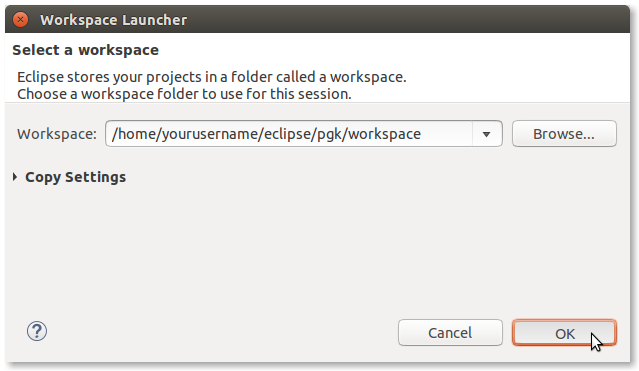
\includegraphics[width=0.8\textwidth]{../img/eclipse/eclipse-select-workspace.png}
\caption {Öppna kursens workspace genom att bläddra till katalogen där du packade upp filen som du laddat ned från: \url{http://cs.lth.se/pgk/ws} \\Om du redan har ett annat workspace öppet, man du växla workspace med menyn \MenuArrow{File}\MenuArrow{Switch Workspace}\Menu{Other...}}
\label{fig:eclipse:ide:open}
\end{figure}

\item
%Stäng välkomstfliken för att komma vidare till workbench (se figur \ref{fig:appendix:eclipse:welcome} på sidan \pageref{fig:appendix:eclipse:welcome}).
Det ska nu se ut ungefär som i figur~\ref{fig:appendix:eclipse:open-perspective} på sidan \pageref{fig:appendix:eclipse:open-perspective}. Det syns ännu inget i \textit{Package Explorer} då vi ännu inte importerat något projekt.

\item Innan du går vidare, säkerställ att du har Scala-perspektivet aktiverat. Du kan växla till Scala-perspektivet genom att trycka på 
\includegraphics[scale=0.75]{../img/eclipse/eclipse-perspective-button.png} eller genom menyn \MenuArrow{Window}\MenuArrow{Perspective}\MenuArrow{Open Perspective}\MenuArrow{Other...}\Menu{Scala}.
%Du kan anpassa inställningarna så att Scala blir \textit{default perspective}, se steg \ref{item:scala-perspective} i avsnitt \ref{subsection:appendix:ide:eclipse:tweaks} på sidan \pageref{subsection:appendix:ide:eclipse:tweaks}.


\item Högerklicka i \textit{Package Explorer} och välj \Menu{Import...}, se Fig.~\ref{fig:eclipse:import}, eller välj menyn \MenuArrow{File}\Menu{Import...}.

\begin{figure}[h]
\centering
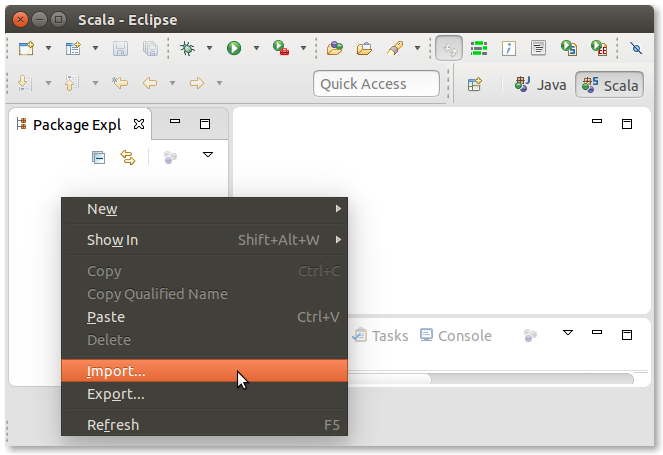
\includegraphics[width=0.9\textwidth]{../img/eclipse/eclipse-import.png}
\caption {Välj \Menu{Import}-menyn för att importera existerande projekt.}
\label{fig:eclipse:import}
\end{figure}

\item Nu öppnas \Menu{Import}-dialogen som visas i figur \ref{fig:eclipse:import-existing}. Öppna mappen \Menu{General}, markera \textbf{Existing Projects into Workspace} och klicka \Button{Next}.



\begin{figure}[h]
\centering
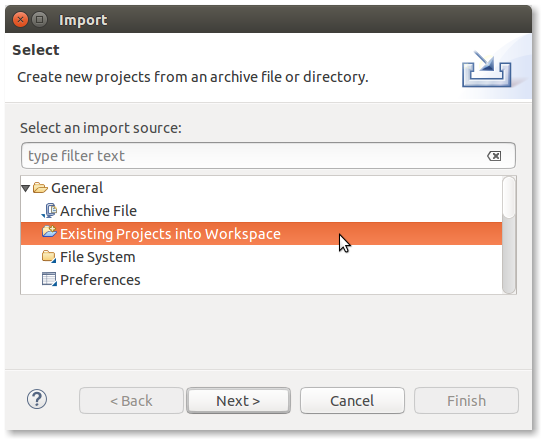
\includegraphics[width=0.6\textwidth]{../img/eclipse/eclipse-import-existing.png}
\caption {Välj att importera existerande projekt under \Menu{General}.}
\label{fig:eclipse:import-existing}
\end{figure}


\begin{figure}[h]
\centering
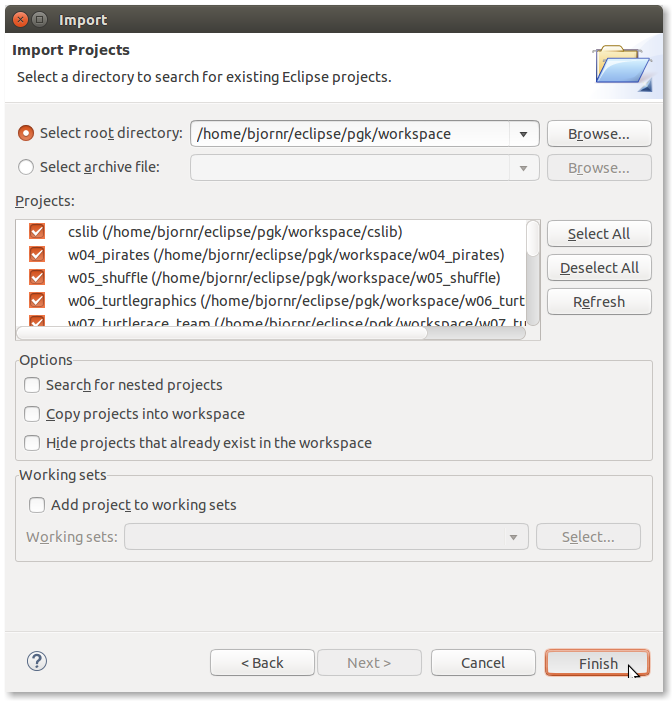
\includegraphics[width=0.85\textwidth]{../img/eclipse/eclipse-import-projects.png}
\caption {Välj \FramedCheckmark{Select Root Directory} (anpassa sökvägen till katalogen där lagt den uppackade katalogen med kursens workspace) och klicka \Button{Browse} och därefter \Button{Ok}. Då kommer katalogerna upp i listan som bilden ovan visar. Alla kataloger ska vara förvalda. Avsluta med att klicka \Button{Finish}}
\label{fig:eclipse:import-projects}
\end{figure}

\item Nu kommer ytterligare ett dialogfönster som visas i figure \ref{fig:eclipse:import-projects}. Följ instruktionerna i bildtexten.

% \item Följ ''Hello World''-instruktionerna på sidan \pageref{subsubsection:eclipse:hello-world} och skapa programmet som visas i figure \ref{fig:eclipse:pirates-hi}, genom att veckla ut projektet \textbf{w04\_pirates}, markera och högerklicka på paketet \textbf{priates}, och välja \MenuArrow{New}\Menu{Scala Object}.

\item Efter att du klickat \Button{Finish} sätter ScalaIDE igång att bygga workspace i bakgrunden. Detta kan ta ett tag. Du kan följa bygget nere till höger i fönstret:
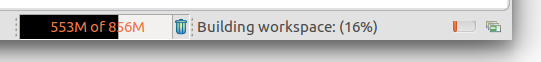
\includegraphics[width=0.75\textwidth]{../img/eclipse/scalaide-import-progress.png}

\item När bygget är klart kan du köra huvudprogrammet i laboration \texttt{w08\_life} genom att högerklicka på filen \texttt{src/main/scala/life/Main.scala} och välja \MenuArrow{Run As}\Menu{Scala Application}.

%\item Om du får problem, fråga någon som känner till Eclipse om hjälp. Det finns även mycket hjälp på nätet, se till exempel: \\ \href{http://stackoverflow.com/questions/8522149/eclipse-not-recognizing-scala-code}{stackoverflow.com/questions/8522149/eclipse-not-recognizing-scala-code}

% \begin{figure}[H]
% \centering
% 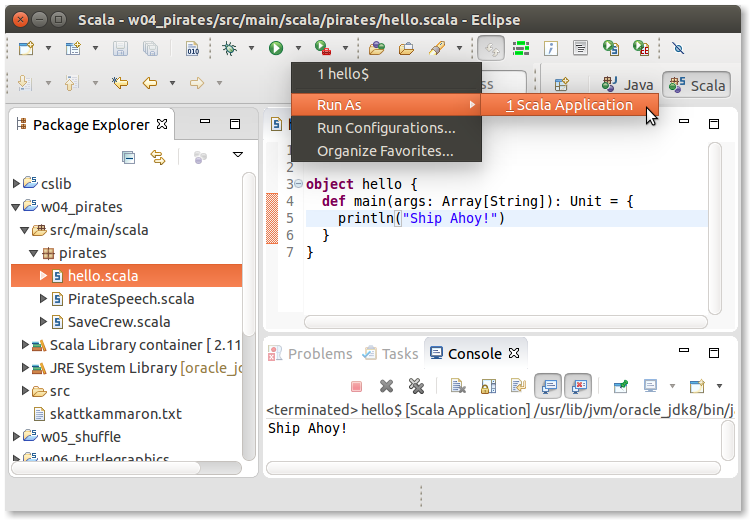
\includegraphics[width=1.0\textwidth]{../img/eclipse/eclipse-pirates-hello.png}
% \caption {Skapa ett \MenuArrow{New}\Menu{Scala Object} med kod enligt bilden.}
% \label{fig:eclipse:pirates-hi}
% \end{figure}


\end{enumerate}

%
% \subsection{Använda debuggern i ScalaIDE/Eclipse}
%
% !!! Läs först appendix \ref{appendix:debug}
%
% \subsubsection{Sätta brytpunkter i Eclipse}\TODO
% \subsubsection{Stegad exekvering i Eclipse}\TODO
% \subsubsection{Inspektera variabler i Eclipse}\TODO

